% Manuscript. Build: cd paper && latexmk main.tex (outputs in build/).
% Numbers come from generated/numbers.tex (python make_numbers.py); references from make_bib.py.
\documentclass[11pt]{article}

% Packages and macros for the manuscript.
\usepackage[T1]{fontenc}
\usepackage[utf8]{inputenc}
\usepackage{lmodern}
\usepackage[margin=2.5cm]{geometry}
\usepackage{setspace}
\usepackage{amsmath}
\usepackage{graphicx}
\usepackage{booktabs}
\usepackage{siunitx}
\usepackage[dvipsnames]{xcolor}
\usepackage[numbers,sort&compress]{natbib}
\usepackage{lineno}
\usepackage{listings}
\usepackage{caption}
\captionsetup[table]{position=top, skip=6pt}
\usepackage{tikz}
\usetikzlibrary{arrows.meta, backgrounds, calc, fit, positioning}
\usepackage[hidelinks]{hyperref}

\graphicspath{{figures/}}
\onehalfspacing
\linenumbers
\lstset{basicstyle=\ttfamily\small, columns=fullflexible, breaklines=true, frame=single,
  framerule=0.3pt, xleftmargin=0.5em, xrightmargin=0.5em}

% Placeholders that stay visible until filled. Search for \result and \todo before submitting.
\newcommand{\result}[1]{\textcolor{orange}{[#1]}}
\newcommand{\todo}[1]{\textcolor{red}{[TODO: #1]}}

% Notation. The app's name is not decided yet; change it here only.
\newcommand{\app}{the app}
\newcommand{\App}{The app}
\newcommand{\setup}[1]{\texttt{#1}}

% \input that works inside tabular and longtable, for generated table rows.
\makeatletter\let\rows\@@input\makeatother

% Numbers generated from eval/results/ by make_numbers.py.
% Generated by make_numbers.py from eval/results/. Do not edit.
\newcommand{\BasePromptTokens}{1,154}
\newcommand{\BaseSeconds}{3.9}
\newcommand{\BaselinePapers}{281}
\newcommand{\BaselinePdfs}{280}
\newcommand{\BaselineQuestions}{1,005}
\newcommand{\CandidateComparisons}{2}
\newcommand{\CiteAllNot}{6.7\% [5.2, 8.5]}
\newcommand{\CiteAllPartial}{15.0\% [12.8, 17.4]}
\newcommand{\CiteAllSupported}{78.4\% [75.6, 80.9]}
\newcommand{\CiteAnswers}{1,002}
\newcommand{\CiteAnswersCiting}{935}
\newcommand{\CiteAnswersCitingRate}{93.3\%}
\newcommand{\CiteHandExact}{39}
\newcommand{\CiteHandKappa}{0.08}
\newcommand{\CiteHandN}{50}
\newcommand{\CiteJudgeNot}{1}
\newcommand{\CiteJudgePartial}{4}
\newcommand{\CiteJudgeRate}{90.0\%}
\newcommand{\CiteJudgeSupported}{45}
\newcommand{\CiteJudged}{915}
\newcommand{\CiteLabellerNot}{6}
\newcommand{\CiteLabellerPartial}{2}
\newcommand{\CiteLabellerRate}{84.0\%}
\newcommand{\CiteLabellerSupported}{42}
\newcommand{\CiteNotJudgedSupported}{6}
\newcommand{\CitePages}{1,588}
\newcommand{\CitePagesInContext}{1,528}
\newcommand{\CitePagesInContextPct}{96.2\%}
\newcommand{\CitePagesInContextRate}{96.2\% [95.2, 97.1]}
\newcommand{\CitePagesOutside}{60}
\newcommand{\CiteStatements}{1,496}
\newcommand{\CiteUnlabelled}{865}
\newcommand{\CompareAppBothCorrect}{21.2\% [14.8, 29.4]}
\newcommand{\CompareAppBothCorrectN}{118}
\newcommand{\CompareAppBothEvidence}{5}
\newcommand{\CompareAppPapersCorrect}{50.4\%}
\newcommand{\CompareAppSlots}{47}
\newcommand{\CompareAppSlotsN}{240}
\newcommand{\CompareBalancedBothCorrect}{28.7\% [21.2, 37.5]}
\newcommand{\CompareBalancedBothCorrectN}{115}
\newcommand{\CompareBalancedBothEvidence}{3}
\newcommand{\CompareBalancedPapersCorrect}{53.9\%}
\newcommand{\CompareBalancedSlots}{43}
\newcommand{\CompareBalancedSlotsN}{240}
\newcommand{\CompareFindableBoth}{83}
\newcommand{\CompareGained}{21}
\newcommand{\CompareLost}{12}
\newcommand{\CompareN}{114}
\newcommand{\CompareP}{0.16}
\newcommand{\ComparePairs}{120}
\newcommand{\ComparePapers}{119}
\newcommand{\ComparePapersFindable}{105}
\newcommand{\CorrectWhenHit}{64.8\% [60.0, 69.4]}
\newcommand{\CorrectWhenHitN}{398}
\newcommand{\CorrectWhenMiss}{42.6\% [38.3, 47.0]}
\newcommand{\CorrectWhenMissN}{493}
\newcommand{\EmptyPdfs}{0}
\newcommand{\Findable}{91.5\% [89.5, 93.1]}
\newcommand{\FindableFifteenHundred}{822}
\newcommand{\FindableFiveHundred}{832}
\newcommand{\FindableK}{815}
\newcommand{\FindableThousand}{815}
\newcommand{\FixedCorrect}{53.6\% [50.5, 56.7]}
\newcommand{\FixedCorrectK}{537}
\newcommand{\FixedCorrectRate}{53.6\%}
\newcommand{\FixedFOne}{11.6}
\newcommand{\FixedN}{1,002}
\newcommand{\FixedPartial}{72.3\% [69.4, 74.9]}
\newcommand{\HitFour}{48.8\% [45.4, 52.3]}
\newcommand{\HitTen}{75.3\%}
\newcommand{\JudgeCheckBinary}{40}
\newcommand{\JudgeCheckClaudeCorrect}{25}
\newcommand{\JudgeCheckExact}{37}
\newcommand{\JudgeCheckHumanBinary}{36}
\newcommand{\JudgeCheckHumanClaudeExact}{32}
\newcommand{\JudgeCheckHumanCorrect}{17}
\newcommand{\JudgeCheckHumanExact}{28}
\newcommand{\JudgeCheckHumanHumanOnly}{2}
\newcommand{\JudgeCheckHumanJudgeOnly}{12}
\newcommand{\JudgeCheckHumanKappa}{0.32}
\newcommand{\JudgeCheckHumanKappaBinary}{0.45}
\newcommand{\JudgeCheckHumanRate}{34.0\% [22.4, 47.8]}
\newcommand{\JudgeCheckHumanRuleBinary}{40}
\newcommand{\JudgeCheckHumanRuleCorrect}{21}
\newcommand{\JudgeCheckHumanRuleExact}{32}
\newcommand{\JudgeCheckHumanRuleHumanOnly}{2}
\newcommand{\JudgeCheckHumanRuleJudgeOnly}{8}
\newcommand{\JudgeCheckHumanRuleKappa}{0.43}
\newcommand{\JudgeCheckHumanRuleKappaBinary}{0.60}
\newcommand{\JudgeCheckHumanRuleRate}{42.0\% [29.4, 55.8]}
\newcommand{\JudgeCheckJudgeCorrect}{27}
\newcommand{\JudgeCheckJudgeRate}{54.0\% [40.4, 67.0]}
\newcommand{\JudgeCheckKappa}{0.57}
\newcommand{\JudgeCheckKappaBinary}{0.60}
\newcommand{\JudgeCheckN}{50}
\newcommand{\JudgeRepeatChangedBinary}{66}
\newcommand{\JudgeRepeatDiff}{0.6}
\newcommand{\JudgeRepeatN}{1,002}
\newcommand{\JudgeRepeatP}{0.54}
\newcommand{\JudgeRepeatSame}{89.2\% [87.1, 91.0]}
\newcommand{\JudgeRepeatSameBinary}{93.4\%}
\newcommand{\JudgeRepeatSameK}{894}
\newcommand{\MedianChunksFifteenHundred}{30}
\newcommand{\MedianChunksFiveHundred}{86}
\newcommand{\MedianChunksThousand}{44}
\newcommand{\MultidocFourMulti}{36.4\% [33.2, 39.8]}
\newcommand{\MultidocFourMultiK}{297}
\newcommand{\MultidocFourMultiLost}{101}
\newcommand{\MultidocFourMultiOwn}{2.59}
\newcommand{\MultidocFourSelected}{48.8\% [45.4, 52.3]}
\newcommand{\MultidocFourSelectedK}{398}
\newcommand{\MultidocFourSelectedLost}{0}
\newcommand{\MultidocFourSelectedOwn}{4.00}
\newcommand{\MultidocFourSingle}{32.3\% [29.1, 35.6]}
\newcommand{\MultidocFourSingleK}{263}
\newcommand{\MultidocFourSingleLost}{135}
\newcommand{\MultidocFourSingleOwn}{2.38}
\newcommand{\MultidocNineMulti}{31.9\% [28.8, 35.2]}
\newcommand{\MultidocNineMultiK}{260}
\newcommand{\MultidocNineMultiLost}{138}
\newcommand{\MultidocNineMultiOwn}{2.23}
\newcommand{\MultidocNineSelected}{48.8\% [45.4, 52.3]}
\newcommand{\MultidocNineSelectedK}{398}
\newcommand{\MultidocNineSelectedLost}{0}
\newcommand{\MultidocNineSelectedOwn}{4.00}
\newcommand{\MultidocNineSingle}{28.1\% [25.1, 31.3]}
\newcommand{\MultidocNineSingleK}{229}
\newcommand{\MultidocNineSingleLost}{169}
\newcommand{\MultidocNineSingleOwn}{2.02}
\newcommand{\MultidocQuestions}{815}
\newcommand{\MultidocTwoMulti}{40.2\% [36.9, 43.7]}
\newcommand{\MultidocTwoMultiK}{328}
\newcommand{\MultidocTwoMultiLost}{70}
\newcommand{\MultidocTwoMultiOwn}{2.91}
\newcommand{\MultidocTwoSelected}{48.8\% [45.4, 52.3]}
\newcommand{\MultidocTwoSelectedK}{398}
\newcommand{\MultidocTwoSelectedLost}{0}
\newcommand{\MultidocTwoSelectedOwn}{4.00}
\newcommand{\MultidocTwoSingle}{37.7\% [34.4, 41.0]}
\newcommand{\MultidocTwoSingleK}{307}
\newcommand{\MultidocTwoSingleLost}{91}
\newcommand{\MultidocTwoSingleOwn}{2.78}
\newcommand{\MultidocZeroMulti}{48.8\% [45.4, 52.3]}
\newcommand{\MultidocZeroMultiK}{398}
\newcommand{\MultidocZeroMultiLost}{0}
\newcommand{\MultidocZeroMultiOwn}{4.00}
\newcommand{\MultidocZeroSelected}{48.8\% [45.4, 52.3]}
\newcommand{\MultidocZeroSelectedK}{398}
\newcommand{\MultidocZeroSelectedLost}{0}
\newcommand{\MultidocZeroSelectedOwn}{4.00}
\newcommand{\MultidocZeroSingle}{48.8\% [45.4, 52.3]}
\newcommand{\MultidocZeroSingleK}{398}
\newcommand{\MultidocZeroSingleLost}{0}
\newcommand{\MultidocZeroSingleOwn}{4.00}
\newcommand{\OracleCorrect}{69.1\% [65.9, 72.0]}
\newcommand{\OracleCorrectK}{616}
\newcommand{\OracleCorrectRate}{69.1\%}
\newcommand{\OracleFOne}{19.0}
\newcommand{\OracleN}{892}
\newcommand{\OraclePartial}{83.9\% [81.3, 86.1]}
\newcommand{\PairedFixedOnOracleQuestions}{52.5\% [49.2, 55.8]}
\newcommand{\PairedOracleGained}{237}
\newcommand{\PairedOracleLost}{90}
\newcommand{\PairedOracleN}{891}
\newcommand{\PairedOracleP}{$2.1 \times 10^{-16}$}
\newcommand{\PapersDownloaded}{280}
\newcommand{\PapersFailed}{1}
\newcommand{\PapersFailedQuestions}{3}
\newcommand{\RepeatFixedChanged}{25.7\%}
\newcommand{\RepeatFixedCorrectInEveryRun}{40.7\%}
\newcommand{\RepeatFixedCorrectInNoRun}{33.6\%}
\newcommand{\RepeatFixedHigh}{54.5\%}
\newcommand{\RepeatFixedIdenticalAnswerTextAllRuns}{1.6\%}
\newcommand{\RepeatFixedLow}{53.2\%}
\newcommand{\RepeatFixedN}{1,000}
\newcommand{\RepeatFixedRates}{53.5, 53.2 and 54.5\%}
\newcommand{\RepeatFixedSameCorrectVsNotAllRuns}{74.3\%}
\newcommand{\RepeatOracleChanged}{23.4\%}
\newcommand{\RepeatOracleCorrectInEveryRun}{57.5\%}
\newcommand{\RepeatOracleCorrectInNoRun}{19.1\%}
\newcommand{\RepeatOracleHigh}{70.9\%}
\newcommand{\RepeatOracleIdenticalAnswerTextAllRuns}{0.2\%}
\newcommand{\RepeatOracleLow}{68.9\%}
\newcommand{\RepeatOracleN}{892}
\newcommand{\RepeatOracleRates}{69.1, 70.9 and 68.9\%}
\newcommand{\RepeatOracleSameCorrectVsNotAllRuns}{76.6\%}
\newcommand{\RepeatOracleVsFixedDiffs}{+16.5, +19.0 and +15.5}
\newcommand{\RepeatOracleVsFixedMaxP}{$5.8 \times 10^{-15}$}
\newcommand{\RepeatOracleVsFixedPs}{$2.1 \times 10^{-16}$, $7.3 \times 10^{-20}$ and $5.8 \times 10^{-15}$}
\newcommand{\RepeatOracleVsFixedSignificantRuns}{3}
\newcommand{\RepeatSmallChanged}{22.1\%}
\newcommand{\RepeatSmallCorrectInEveryRun}{45.7\%}
\newcommand{\RepeatSmallCorrectInNoRun}{32.3\%}
\newcommand{\RepeatSmallHigh}{57.1\%}
\newcommand{\RepeatSmallIdenticalAnswerTextAllRuns}{3.3\%}
\newcommand{\RepeatSmallLow}{55.7\%}
\newcommand{\RepeatSmallN}{1,001}
\newcommand{\RepeatSmallRates}{57.1, 55.7 and 56.2\%}
\newcommand{\RepeatSmallRerankChanged}{27.5\%}
\newcommand{\RepeatSmallRerankCorrectInEveryRun}{43.3\%}
\newcommand{\RepeatSmallRerankCorrectInNoRun}{29.3\%}
\newcommand{\RepeatSmallRerankHigh}{59.3\%}
\newcommand{\RepeatSmallRerankIdenticalAnswerTextAllRuns}{2.6\%}
\newcommand{\RepeatSmallRerankLow}{55.7\%}
\newcommand{\RepeatSmallRerankN}{994}
\newcommand{\RepeatSmallRerankRates}{56.6, 59.3 and 55.7\%}
\newcommand{\RepeatSmallRerankSameCorrectVsNotAllRuns}{72.5\%}
\newcommand{\RepeatSmallRerankVsFixedDiffs}{+3.0, +5.9 and +1.4}
\newcommand{\RepeatSmallRerankVsFixedMaxP}{0.43}
\newcommand{\RepeatSmallRerankVsFixedPs}{0.095, $5.9 \times 10^{-4}$ and 0.43}
\newcommand{\RepeatSmallRerankVsFixedSignificantRuns}{1}
\newcommand{\RepeatSmallSameCorrectVsNotAllRuns}{77.9\%}
\newcommand{\RepeatSmallVsFixedDiffs}{+3.5, +2.5 and +1.8}
\newcommand{\RepeatSmallVsFixedMaxP}{0.3}
\newcommand{\RepeatSmallVsFixedPs}{0.035, 0.14 and 0.3}
\newcommand{\RepeatSmallVsFixedSignificantRuns}{1}
\newcommand{\RepeatWidestGained}{113}
\newcommand{\RepeatWidestLost}{78}
\newcommand{\RepeatWidestP}{0.014}
\newcommand{\RepeatWidestPoints}{3.5}
\newcommand{\RepeatWidestSetup}{500 / top 8, reranked}
\newcommand{\RerankAddedCorrectAfter}{58}
\newcommand{\RerankAddedCorrectBefore}{47}
\newcommand{\RerankAddedN}{111}
\newcommand{\RerankRemovedCorrectAfter}{29}
\newcommand{\RerankRemovedCorrectBefore}{31}
\newcommand{\RerankRemovedN}{54}
\newcommand{\RerankSameGained}{87}
\newcommand{\RerankSameLost}{101}
\newcommand{\RerankSameN}{837}
\newcommand{\RerankVsSmallGained}{114}
\newcommand{\RerankVsSmallLost}{119}
\newcommand{\RerankVsSmallP}{0.79}
\newcommand{\RetryAnswersAfter}{54.8\% [51.7, 57.8]}
\newcommand{\RetryAnswersAfterRate}{54.8\%}
\newcommand{\RetryAnswersBefore}{53.6\% [50.5, 56.7]}
\newcommand{\RetryAnswersBeforeRate}{53.6\%}
\newcommand{\RetryAnswersGained}{91}
\newcommand{\RetryAnswersLost}{79}
\newcommand{\RetryAnswersN}{1,002}
\newcommand{\RetryAnswersP}{0.4}
\newcommand{\RetryChecked}{1,005}
\newcommand{\RetryHeld}{398}
\newcommand{\RetryHeldRetried}{29}
\newcommand{\RetryHitAfter}{45.0\% [41.8, 48.3]}
\newcommand{\RetryHitAfterRate}{45.0\%}
\newcommand{\RetryHitBefore}{44.7\% [41.4, 47.9]}
\newcommand{\RetryHitBeforeRate}{44.7\%}
\newcommand{\RetryHitGained}{13}
\newcommand{\RetryHitLost}{10}
\newcommand{\RetryHitN}{891}
\newcommand{\RetryHitP}{0.68}
\newcommand{\RetryMissed}{493}
\newcommand{\RetryMissedKept}{396}
\newcommand{\RetryMissedKeptRate}{80.3\%}
\newcommand{\RetryN}{177}
\newcommand{\RetryRate}{17.6\%}
\newcommand{\RetryRetriedAfter}{102}
\newcommand{\RetryRetriedBefore}{94}
\newcommand{\SectionsAnswersAfter}{54.5\% [51.4, 57.6]}
\newcommand{\SectionsAnswersAfterRate}{54.5\%}
\newcommand{\SectionsAnswersBefore}{53.6\% [50.5, 56.7]}
\newcommand{\SectionsAnswersBeforeRate}{53.6\%}
\newcommand{\SectionsAnswersGained}{139}
\newcommand{\SectionsAnswersLost}{130}
\newcommand{\SectionsAnswersN}{1,002}
\newcommand{\SectionsAnswersP}{0.63}
\newcommand{\SectionsCoverage}{80.6\%}
\newcommand{\SectionsCoverageK}{2,919}
\newcommand{\SectionsCoverageN}{3,621}
\newcommand{\SectionsHitAfter}{47.5\% [44.2, 50.8]}
\newcommand{\SectionsHitAfterRate}{47.5\%}
\newcommand{\SectionsHitBefore}{44.7\% [41.4, 47.9]}
\newcommand{\SectionsHitBeforeRate}{44.7\%}
\newcommand{\SectionsHitGained}{117}
\newcommand{\SectionsHitLost}{92}
\newcommand{\SectionsHitN}{891}
\newcommand{\SectionsHitP}{0.097}
\newcommand{\SectionsSmallHitAfter}{55.4\% [52.2, 58.7]}
\newcommand{\SectionsSmallHitAfterRate}{55.4\%}
\newcommand{\SectionsSmallHitBefore}{53.8\% [50.5, 57.0]}
\newcommand{\SectionsSmallHitBeforeRate}{53.8\%}
\newcommand{\SectionsSmallHitGained}{94}
\newcommand{\SectionsSmallHitLost}{79}
\newcommand{\SectionsSmallHitN}{891}
\newcommand{\SectionsSmallHitP}{0.29}
\newcommand{\ShippedCorrect}{0.0\% [0.0, 0.4]}
\newcommand{\ShippedCorrectK}{0}
\newcommand{\ShippedCorrectRate}{0.0\%}
\newcommand{\ShippedEmpty}{1,005}
\newcommand{\ShippedFOne}{0.0}
\newcommand{\ShippedN}{1,005}
\newcommand{\ShippedPartial}{0.0\% [0.0, 0.4]}
\newcommand{\SmallCorrect}{57.1\% [54.0, 60.1]}
\newcommand{\SmallCorrectRate}{57.1\%}
\newcommand{\SmallCorrectWhenHit}{64.1\%}
\newcommand{\SmallCorrectWhenMiss}{46.4\%}
\newcommand{\SmallFindableK}{832}
\newcommand{\SmallGained}{148}
\newcommand{\SmallHitEight}{57.6\% [54.2, 60.9]}
\newcommand{\SmallHolmP}{0.07}
\newcommand{\SmallLost}{113}
\newcommand{\SmallNotJudged}{1}
\newcommand{\SmallPairedN}{1,002}
\newcommand{\SmallPartial}{75.2\%}
\newcommand{\SmallPromptTokens}{1,230}
\newcommand{\SmallRerankCorrect}{56.6\% [53.5, 59.6]}
\newcommand{\SmallRerankCorrectRate}{56.6\%}
\newcommand{\SmallRerankCorrectWhenHit}{61.6\%}
\newcommand{\SmallRerankCorrectWhenMiss}{48.5\%}
\newcommand{\SmallRerankGained}{166}
\newcommand{\SmallRerankHitEight}{64.4\% [61.1, 67.6]}
\newcommand{\SmallRerankHolmP}{0.095}
\newcommand{\SmallRerankLost}{136}
\newcommand{\SmallRerankNotJudged}{0}
\newcommand{\SmallRerankPairedN}{1,002}
\newcommand{\SmallRerankPartial}{75.9\%}
\newcommand{\SmallRerankPromptTokens}{1,197}
\newcommand{\SmallRerankSeconds}{4.5}
\newcommand{\SmallSeconds}{7.1}
\newcommand{\SweepBaseBudget}{49.4\% [45.9, 52.9]}
\newcommand{\SweepBaseBudgetRate}{49.4\%}
\newcommand{\SweepBaseHitFour}{49.4\% [45.9, 52.9]}
\newcommand{\SweepBestBudget}{65.9\% [62.5, 69.1]}
\newcommand{\SweepBestBudgetRate}{65.9\%}
\newcommand{\SweepBestGained}{207}
\newcommand{\SweepBestHitFour}{51.3\% [47.8, 54.8]}
\newcommand{\SweepBestLost}{78}
\newcommand{\SweepBestName}{\texttt{c500/rerank-hybrid-bge}}
\newcommand{\SweepBestP}{$4.0 \times 10^{-13}$}
\newcommand{\SweepBigHybridBudget}{57.0\% [53.5, 60.5]}
\newcommand{\SweepBigHybridBudgetRate}{57.0\%}
\newcommand{\SweepBigHybridGained}{158}
\newcommand{\SweepBigHybridHitFour}{64.7\% [61.3, 68.0]}
\newcommand{\SweepBigHybridLost}{98}
\newcommand{\SweepBigHybridP}{0.004}
\newcommand{\SweepComparisons}{35}
\newcommand{\SweepQuestions}{782}
\newcommand{\SweepSetups}{36}
\newcommand{\SweepSmallBudget}{58.4\% [55.0, 61.8]}
\newcommand{\SweepSmallBudgetRate}{58.4\%}
\newcommand{\SweepSmallGained}{139}
\newcommand{\SweepSmallHitFour}{43.5\% [40.0, 47.0]}
\newcommand{\SweepSmallLost}{68}
\newcommand{\SweepSmallP}{$2.3 \times 10^{-5}$}
\newcommand{\SweepSmallRerankBudget}{65.5\% [62.1, 68.7]}
\newcommand{\SweepSmallRerankBudgetRate}{65.5\%}
\newcommand{\SweepSmallRerankGained}{194}
\newcommand{\SweepSmallRerankHitFour}{49.9\% [46.4, 53.4]}
\newcommand{\SweepSmallRerankLost}{68}
\newcommand{\SweepSmallRerankP}{$1.1 \times 10^{-13}$}
\newcommand{\TextEvidenceQuestions}{891}



% Working title (ROADMAP.md): "reliability" needs the repeat-run and citation-check experiments,
% and "beyond retrieval" is revisited if an improvement in the planned section works clearly.
\title{Beyond retrieval: evaluating the reliability of retrieval-augmented question answering
  over scientific papers}
\author{David Obeh Alobo\\
  \small University of Glasgow\\
  \small \texttt{2941522A@student.gla.ac.uk}}
\date{}

\begin{document}
\maketitle

\begin{abstract}
Question answering over a PDF with retrieval-augmented generation is a common small project:
split the document into chunks, embed them, retrieve the most similar few and pass them to a
language model. Such apps are rarely measured. We took one, an open-source Streamlit app for
research papers, and evaluated its own code on the 1,005 questions of the QASPER development
set, using the arXiv PDFs of the 281 papers, Llama~3.1~8B as the answering model and Qwen3-32B
as a judge checked against blind hand labels. As shipped, a misplaced loop sent the first
question of every conversation to the model without the question or the document; the model
returned \result{N} empty answers out of 1,005. After the fix, \result{X\%} of answers were
judged correct, against \result{Y\%} when the model was given the annotators' own evidence
paragraphs. At equal prompt length (about 4,000 characters), 500-character chunks with
cross-encoder reranking put a gold evidence passage in the context for \SweepSmallRerankBudget{}
of \SweepQuestions{} questions, against \SweepBaseBudget{} for the app's 1,000-character
chunks; on answers this \result{raised correctness to Z\%}. Loading nine other papers alongside
the one a question is about lowered evidence retrieval from \MultidocZeroSingle{} to
\MultidocNineMulti{}; letting the user restrict the search to one paper restored it. All code,
per-question outputs and prompts are released.
\end{abstract}


\section{Introduction}
\label{sec:intro}

Retrieval-augmented generation~\cite{lewis2020rag} allows a language model to answer questions
from a document it was not trained on. For a single PDF, the usual approach is simple. The text is
split into chunks of a fixed number of characters, each chunk is embedded with a sentence encoder
such as Sentence-BERT~\cite{reimers2019sbert}, the chunks nearest to the question are found in a
vector index, and these are sent to the model together with the question. This approach is used
in many tutorials, course projects and portfolio repositories. A common configuration, which is
also the one in our app, is 1,000-character chunks, the MiniLM encoder~\cite{wang2020minilm}, a
FAISS index~\cite{johnson2021faiss} and the top four chunks. Such apps are rarely tested on a
public benchmark. When they are, the report usually covers either retrieval or the answers, and
does not show where between the two the answers are lost.

Research systems for scientific question answering are evaluated more carefully, but they are
built differently. PaperQA~\cite{lala2023paperqa} and PaperQA2~\cite{skarlinski2024paperqa2}
search the literature, summarise each retrieved passage for the question before answering, and
may decline to answer. OpenScholar~\cite{asai2024openscholar} retrieves from tens of millions of
papers and revises its answers using feedback. These systems answer questions across the
literature, whereas the small apps answer questions about a paper the user already has. This is
the setting of the QASPER benchmark~\cite{dasigi2021qasper}, in which questions were written by
readers who had seen only the title and abstract of an NLP paper, and answered by other
annotators from the full text, who also marked the evidence paragraphs.

We built one such app, CitePage, which answers questions about uploaded PDFs through the Groq
API, and in this paper we run its own pipeline over the QASPER development set. We first wanted
to know how the app behaved as we had released it, and how often retrieval, rather than the
model, was what kept an answer from being right. We then tried the settings people usually
change (chunk size, embedding model, keyword search and reranking) while keeping the prompt the
same length. Users also load several papers at once, so we checked whether retrieval still finds
the paper a question is about. Finally, we checked the measurements themselves. We graded a
sample of answers by hand to see how far to trust the language-model judge, asked every question
three times to see how much the results move, and looked at whether the pages an answer cites
contain what it says.

These results come from one app, one benchmark of NLP papers and one answering model, and we
do not propose a new method. Instead, we show where a typical pipeline loses its answers, and
which of the changes we tried helped and which did not. Every number in the paper can be traced
to the per-question outputs we release.

\section{The app}
\label{sec:app}

\App{} is a Streamlit web application written in Python. A user uploads a PDF and asks questions
in a chat. The PDF is read page by page with pypdf through LangChain's \texttt{PyPDFLoader} and
split by LangChain's recursive character splitter into chunks of at most 1,000 characters with
200 characters of overlap. Each chunk is embedded locally with all-MiniLM-L6-v2 and stored in a
flat FAISS index. For each question the four nearest chunks are retrieved and sent, with a
system prompt and the recent conversation, to a model on the Groq API; Llama~3.1~8B is the
default. Only the retrieved chunks and the conversation leave the user's machine
(Fig.~\ref{fig:system}a).

% Figure 1: the app's pipeline (a) and the message bug (b). Drawn in TikZ on a fixed grid; the
% numbers are the app's defaults as described in sections/app.tex.
\begin{figure}[t]
\centering
\hyphenpenalty=10000
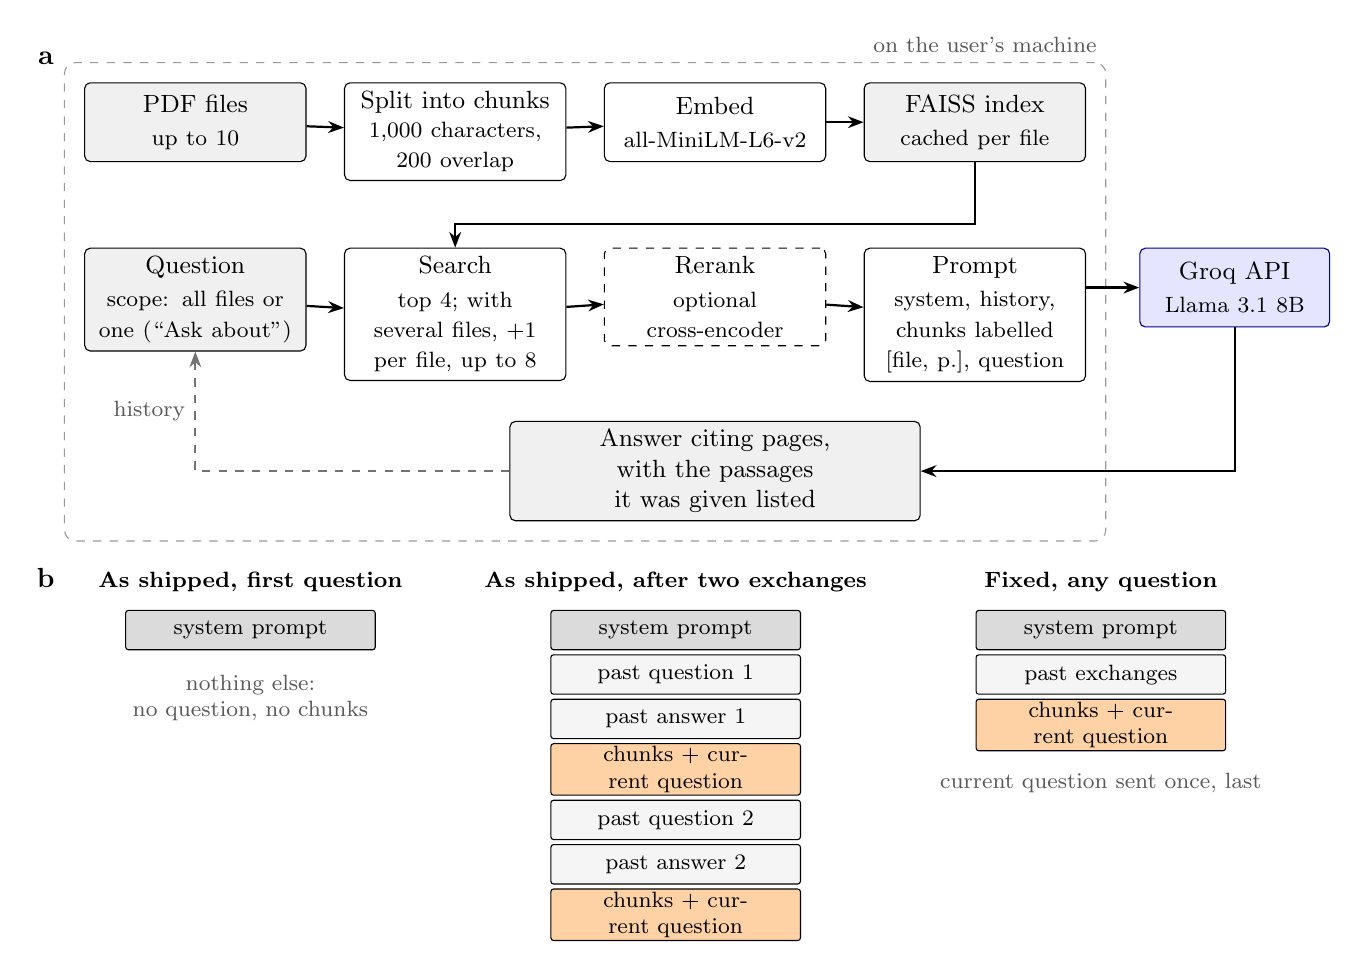
\begin{tikzpicture}[
  font=\small,
  box/.style={draw, rounded corners=2pt, align=center, inner sep=3pt, minimum height=10mm,
    text width=#1, anchor=north},
  box/.default=26mm,
  data/.style={box=#1, fill=black!6},
  data/.default=26mm,
  remote/.style={box=#1, fill=blue!10, draw=blue!60!black},
  remote/.default=22mm,
  arr/.style={-{Stealth[length=2mm]}, thick},
  note/.style={font=\footnotesize, align=center, text=black!65},
  sub/.style={font=\footnotesize},
]
% --- (a) pipeline -------------------------------------------------------------------------
\node[font=\bfseries] at (-0.6, 0.3) {a};

% Indexing, once per file
\node[data] (pdf) at (1.3, 0) {PDF files\\[1pt]\footnotesize up to 10};
\node[box] (split) at (4.6, 0) {Split into chunks\\[1pt]\footnotesize 1,000 characters,\\200 overlap};
\node[box] (embed) at (7.9, 0) {Embed\\[1pt]\footnotesize all-MiniLM-L6-v2};
\node[data] (index) at (11.2, 0) {FAISS index\\[1pt]\footnotesize cached per file};
\draw[arr] (pdf) -- (split);
\draw[arr] (split) -- (embed);
\draw[arr] (embed) -- (index);

% Answering, once per question
\node[data] (q) at (1.3, -2.1) {Question\\[1pt]\footnotesize scope: all files or one (``Ask about'')};
\node[box] (search) at (4.6, -2.1) {Search\\[1pt]\footnotesize top 4; with several files, +1 per file, up to 8};
\node[box, dashed] (rerank) at (7.9, -2.1) {Rerank\\[1pt]\footnotesize optional cross-encoder};
\node[box] (prompt) at (11.2, -2.1) {Prompt\\[1pt]\footnotesize system, history, chunks labelled [file, p.], question};
\draw[arr] (q) -- (search);
\draw[arr] (search) -- (rerank);
\draw[arr] (rerank) -- (prompt);
\coordinate (gap) at (0, -1.8);
\draw[arr] (index.south) -- (index.south |- gap) -- (search.north |- gap) -- (search.north);

\node[remote] (llm) at (14.5, -2.1) {Groq API\\[1pt]\footnotesize Llama~3.1~8B};
\node[data=50mm] (answer) at (7.9, -4.3) {Answer citing pages,\\with the passages it was given listed};
\draw[arr] (prompt.east |- llm.west) -- (llm.west);
\draw[arr] (llm.south) |- (answer.east);
\draw[arr, dashed, black!55] (answer.west) -| node[note, pos=0.75, left] {history} (q.south);

% What stays local
\begin{scope}[on background layer]
  \node[draw=black!40, dashed, rounded corners=4pt, inner sep=2.5mm,
    fit=(pdf) (index) (q) (prompt) (answer)] (local) {};
\end{scope}
\node[note, anchor=south east] at (local.north east) {on the user's machine};

% --- (b) the message bug -------------------------------------------------------------------
\begin{scope}[yshift=-6.6cm,
  msg/.style={draw, rounded corners=1pt, text width=31mm, align=center, minimum height=5mm,
    inner sep=1pt, font=\footnotesize, anchor=north},
  sys/.style={msg, fill=black!14},
  past/.style={msg, fill=black!4},
  cur/.style={msg, fill=orange!35},
  head/.style={font=\footnotesize\bfseries, anchor=south}]
\node[font=\bfseries] at (-0.6, 0.3) {b};

\node[head] at (2.0, 0) {As shipped, first question};
\node[sys] (s1) at (2.0, -0.1) {system prompt};
\node[note, anchor=north] at (2.0, -0.8) {nothing else:\\no question, no chunks};

\node[head] at (7.4, 0) {As shipped, after two exchanges};
\node[sys] (s2) at (7.4, -0.1) {system prompt};
\node[past, below=0.5mm of s2] (p1) {past question 1};
\node[past, below=0.5mm of p1] (a1) {past answer 1};
\node[cur, below=0.5mm of a1] (c1) {chunks + current question};
\node[past, below=0.5mm of c1] (p2) {past question 2};
\node[past, below=0.5mm of p2] (a2) {past answer 2};
\node[cur, below=0.5mm of a2] (c2) {chunks + current question};

\node[head] at (12.8, 0) {Fixed, any question};
\node[sys] (s3) at (12.8, -0.1) {system prompt};
\node[past, below=0.5mm of s3] (h1) {past exchanges};
\node[cur, below=0.5mm of h1] (c3) {chunks + current question};
\node[note, below=1.5mm of c3] {current question sent once, last};
\end{scope}
\end{tikzpicture}
\caption{\textbf{a}, \App{} after the fixes. Each file is split, embedded and indexed once. Each
question is searched in the index, or in one file's chunks when the user picks it under ``Ask
about'', and the retrieved chunks, labelled with file and page, go to the language model with
the system prompt and recent conversation. Only the prompt leaves the user's machine. The
reranker is optional. \textbf{b}, The messages sent to the model. As shipped, the code that adds
the chunks and the question sat inside the loop over past exchanges, so the first question was
sent as the system prompt alone, and later questions were repeated once per past exchange.}
\label{fig:system}
\end{figure}


\subsection{Defects found}
\label{sec:defects}

Reading the code and running the app found four defects in the version on the main branch
(commit \texttt{5a48041}).

\begin{enumerate}
  \item \textbf{The current question was built inside the loop over past exchanges.} The code
  that appends the retrieved chunks and the question to the messages was indented one level too
  deep, inside the loop that adds previous exchanges. With no previous exchange, the loop body
  never ran and the model received the system prompt alone, with neither the question nor the
  document. With $h$ previous exchanges (up to five) it received the question and its context
  $h$ times, interleaved with the history (Fig.~\ref{fig:system}b).
  \item \textbf{History trimming returned one exchange, not a list.} Once the history held more
  than ten exchanges, the function meant to keep the last ten returned the tenth from last as a
  single (question, answer) pair. Iterating over it then failed, so from the twelfth question of
  a conversation every question ended in an error message.
  \item \textbf{An unreadable PDF was treated as text.} The loader returned the error message as
  a string where a list of chunks was expected, and the next step failed on it.
  \item \textbf{Streamlit reruns repeated work and questions.} The script reruns on every
  interaction. The PDF was embedded again for each question, and because the question box kept
  its text, any later click (for instance on ``clear history'') asked the last question again
  and added it to the history once more.
\end{enumerate}

None of these raised an error on the first question, which is the only one most people try. The
first defect also does not show as an error: the model receives a valid request and replies, in
our runs with an empty answer (Section~\ref{sec:res-shipped}).

\subsection{Changes}
\label{sec:changes}

We fixed the four defects, each with a regression test, and made three changes that the
evaluation in this paper motivated or measured. Every answer now lists the passages it was
given, with their pages, and the prompt asks the model to cite pages. Several PDFs can be
loaded at once; each is embedded once and cached, and passages are labelled with their file.
With several files, retrieval takes the top four chunks and then the best chunk of each file not
yet represented, up to eight, so that a question comparing the papers sees all of them; an
``Ask about'' control restricts the search to one file (Section~\ref{sec:res-multidoc}).
The retrieval defaults (1,000-character chunks, top four) are unchanged: the set-ups that
retrieved evidence more often did not answer detectably better
(Section~\ref{sec:res-candidates}).

\section{Evaluation}
\label{sec:evaluation}

Figure~\ref{fig:evaluation} gives an overview of the experiments.

% Figure 2: the evaluation design, on a fixed grid. Counts come from generated/numbers.tex.
\begin{figure}[t]
\centering
\hyphenpenalty=10000
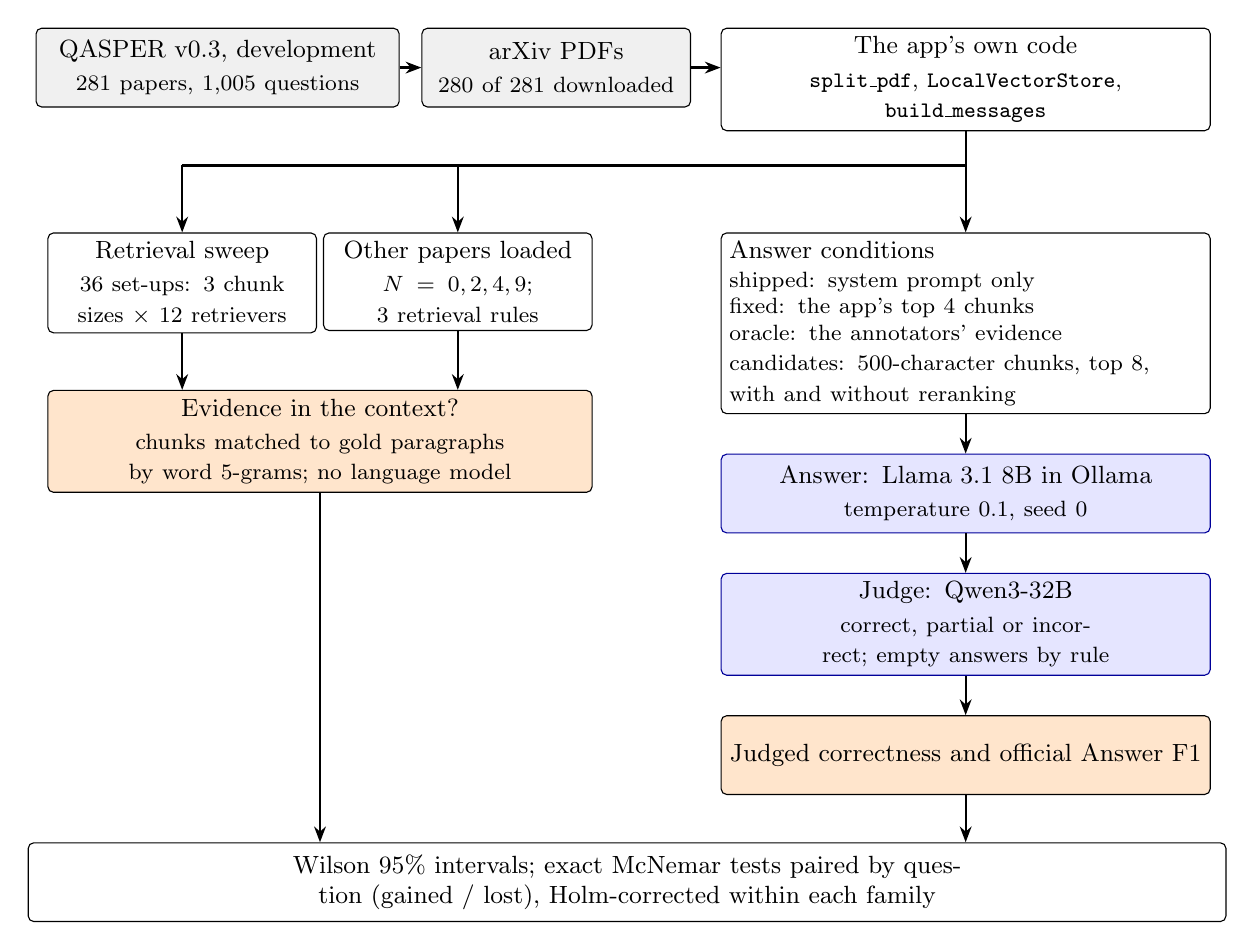
\begin{tikzpicture}[
  font=\small,
  box/.style={draw, rounded corners=2pt, align=center, inner sep=3pt, minimum height=10mm,
    text width=#1, anchor=north},
  box/.default=32mm,
  data/.style={box=#1, fill=black!6},
  data/.default=32mm,
  model/.style={box=#1, fill=blue!10, draw=blue!60!black},
  model/.default=60mm,
  out/.style={box=#1, fill=orange!20},
  out/.default=60mm,
  arr/.style={-{Stealth[length=2mm]}, thick},
]
% Inputs
\node[data=44mm] (qasper) at (2.3, 0) {QASPER v0.3, development\\[1pt]\footnotesize
  \BaselinePapers{} papers, \BaselineQuestions{} questions};
\node[data] (pdfs) at (6.6, 0) {arXiv PDFs\\[1pt]\footnotesize \BaselinePdfs{} of \BaselinePapers{} downloaded};
\node[box=60mm] (app) at (11.8, 0) {The app's own code\\[1pt]\footnotesize
  \texttt{split\_pdf}, \texttt{LocalVectorStore}, \texttt{build\_messages}};
\draw[arr] (qasper.east |- pdfs.west) -- (pdfs.west);
\draw[arr] (pdfs.east) -- (pdfs.east -| app.west);

% Retrieval only (no language model)
\node[box] (sweep) at (1.85, -2.6) {Retrieval sweep\\[1pt]\footnotesize \SweepSetups{} set-ups:
  3 chunk sizes $\times$ 12 retrievers};
\node[box] (multi) at (5.35, -2.6) {Other papers loaded\\[1pt]\footnotesize $N = 0, 2, 4, 9$;
  3 retrieval rules};
\node[out=67mm] (match) at (3.6, -4.6) {Evidence in the context?\\[1pt]\footnotesize chunks
  matched to gold paragraphs by word 5-grams; no language model};
\draw[arr] (sweep.south) -- (sweep.south |- match.north);
\draw[arr] (multi.south) -- (multi.south |- match.north);

% Answers
\node[box=60mm, align=left] (conds) at (11.8, -2.6) {Answer conditions\\[1pt]\footnotesize
  shipped: system prompt only\\
  fixed: the app's top 4 chunks\\
  oracle: the annotators' evidence\\
  candidates: 500-character chunks, top 8, with and without reranking};
\node[model, below=5mm of conds] (llm) {Answer: Llama~3.1~8B in Ollama\\[1pt]\footnotesize
  temperature 0.1, seed 0};
\node[model, below=5mm of llm] (judge) {Judge: Qwen3-32B\\[1pt]\footnotesize correct, partial or
  incorrect; empty answers by rule};
\node[out, below=5mm of judge] (f1) {Judged correctness and official Answer F1};
\draw[arr] (conds) -- (llm);
\draw[arr] (llm) -- (judge);
\draw[arr] (judge) -- (f1);

% From the app's code to both branches
\coordinate (bus) at (0, -1.75);
\draw[thick] (app.south) -- (app.south |- bus);
\draw[thick] (sweep.north |- bus) -- (app.south |- bus);
\draw[arr] (sweep.north |- bus) -- (sweep.north);
\draw[arr] (multi.north |- bus) -- (multi.north);
\draw[arr] (app.south |- bus) -- (conds.north);

% Statistics
\path (f1.south) ++(0, -6mm) coordinate (statsy);
\coordinate (mid) at (7.5, 0);
\node[box=150mm] (stats) at (mid |- statsy) {Wilson 95\% intervals; exact McNemar tests paired by
  question (gained / lost), Holm-corrected within each family};
\draw[arr] (match.south) -- (match.south |- stats.north);
\draw[arr] (f1.south) -- (f1.south |- stats.north);
\end{tikzpicture}
\caption{Evaluation design. Every experiment runs the app's own retrieval and prompting code on
the arXiv PDFs of the QASPER development papers. Retrieval experiments score whether a gold
evidence paragraph reached the context, without calling a language model; answer experiments
generate with Llama~3.1~8B and grade with a Qwen3-32B judge and the official Answer F1.
Comparisons are paired by question.}
\label{fig:evaluation}
\end{figure}


\subsection{Data}

We used the development split of QASPER v0.3~\cite{dasigi2021qasper}, which contains 281 NLP
papers and 1,005 questions. Each question was answered by one or more annotators, who also
marked the paragraphs that hold the evidence. We kept the test split for a final comparison once
the design is settled. Because the app reads PDFs and not the dataset's parsed text, we
downloaded each paper from arXiv, with one request every three seconds as arXiv asks of automated
clients. 280 of the 281 downloads succeeded. The current arXiv version of a paper may differ from
the one QASPER was built from, and we measure the effect of this through evidence findability
(below).

\subsection{Pipeline under test}

All retrieval and prompting used the app's own functions (\texttt{Utils.split\_pdf},
\texttt{LocalVectorStore} and \texttt{Utils.build\_messages}). The only difference from the app
is that the model ran in Ollama instead of on Groq, behind a client with the same interface, so
that every run could be repeated on our own hardware. We used \texttt{llama3.1:8b}, which has the
same weights as Groq's \texttt{llama-3.1-8b-instant}, in Ollama's 4-bit Q4\_K\_M quantization.
This may answer slightly differently from Groq's deployment. Generation used the app's settings
(temperature 0.1 and at most 1,000 tokens), with seed 0 and a 16,384-token context window, which
is larger than any prompt in the evaluation. Each question was asked on its own, without
conversation history.

We compared three conditions. \emph{Shipped} sends what the app sent for the first question of a
conversation before the fix, which is the system prompt alone. \emph{Fixed} sends the fixed app's
prompt with the four retrieved chunks. \emph{Oracle} sends the same prompt with the annotators'
evidence paragraphs in place of the retrieved chunks. The oracle condition shows how well this
model and prompt could do if retrieval were perfect.

\subsection{Evidence retrieval}
\label{sec:ev-evidence}

We scored retrieval by whether a chunk holding a gold evidence paragraph was among the chunks
sent to the model. QASPER's paragraphs come from a parse of the paper's source, while the chunks
come from the PDF text, so the two had to be matched approximately. Both were normalised
(Unicode NFKC, line-break hyphens removed, lower case and alphanumeric tokens only). A chunk was
taken to hold a paragraph if it contained at least half of the paragraph's word 5-grams, or, for
paragraphs longer than a chunk, if at least half of the chunk's own 5-grams were in the
paragraph. We call a question's evidence \emph{findable} if some chunk of the whole PDF holds it,
and we compute retrieval rates over the questions with findable evidence. As in QASPER's
text-only evidence, figures and tables are left out.

\subsection{Retrieval sweep}

To choose retrieval settings without calling a language model, we ranked every paper's chunks for
every question under \SweepSetups{} set-ups. These covered three chunk sizes (500, 1,000 and
1,500 characters, with 20\% overlap) and several retrievers: dense retrieval with
all-MiniLM-L6-v2~\cite{wang2020minilm}, bge-small-en-v1.5~\cite{xiao2023cpack} or
e5-small-v2~\cite{wang2022e5}; BM25 keyword search~\cite{robertson2009bm25}; and hybrids of the
dense and BM25 rankings by reciprocal rank fusion~\cite{cormack2009rrf}. Five of these (MiniLM,
BM25 and the three hybrids) were also run with their top 20 chunks reranked by a cross-encoder
trained on MS~MARCO~\cite{nogueira2019rerank,bajaj2016msmarco}
(\texttt{cross-encoder/ms-marco-MiniLM-L-6-v2}). Four chunks of 1,500 characters hold three
times as much text as four chunks of 500, so we compared the set-ups at the same budget of about
4,000 characters, which is the top 8, 4 or 3 chunks depending on the chunk size. The comparison
uses the \SweepQuestions{} questions whose evidence is findable at every chunk size.

\subsection{Several papers}

To test whether other papers crowd out the one a question is about, we loaded each paper into the
app's vector store together with 2, 4 or 9 other development papers drawn at random (seed 0). We
then searched with three rules: the top four chunks; the app's rule for several files, which takes
the top four and then one chunk from each file not yet represented, up to eight; and the top four
chunks of the question's own paper, which is what happens when the user selects that paper under
``Ask about''.

\subsection{Judging answers}

We graded the answers in two ways. The official QASPER evaluator computes token F1 against each
annotator's answer and keeps the best score. It suits short extractive answers but penalises the
app's full-sentence answers, so we report it without relying on it. Our main measure was a
judgement by Qwen3-32B~\cite{yang2025qwen3} (Q4\_K\_M, reasoning enabled, temperature 0). The
judge was given the question, every annotator's answer and the app's answer, and asked whether
the app's answer gives the substance of at least one reference answer (correct), part of it
(partially correct) or neither (incorrect). The prompt is in the SI. Language-model judges have
known biases~\cite{zheng2023judge}, and in a pilot on nine answers our judge gave credit to empty
answers. We therefore graded empty answers as incorrect by rule. Three of the fixed app's
judgements came back empty because the judge's reasoning filled its 8,192-token window. These
were graded again with a 20,480-token window, and both attempts are kept.

To check the judge, we drew \JudgeCheckN{} answers of the fixed app at random (seed 0). Claude
(Anthropic) first graded them with the judge's rules, before any of the judge's verdicts on them
had been read (Section~\ref{sec:res-judge}). We then labelled the same answers ourselves, without
seeing the judge's verdicts or Claude's labels, on a page that showed the question, the reference
answers and the app's answer together with the judge's instructions (SI, Section~S6). Like the
judge, neither Claude nor we read the papers, and all grading was done against the references.

\subsection{Repeat runs}
\label{sec:eval-repeats}

Because the app answers at temperature 0.1, the same question can get a different answer in
another run. To measure how much this changes the results, we answered every question twice more
for each of the four set-ups compared in Section~\ref{sec:results} (the fixed app, the
annotators' evidence and the two leading retrieval set-ups). These runs used answer-model seeds 1
and 2 and were judged as before, and the original runs count as seed 0. Retrieval is
deterministic, so it was not repeated and the saved chunks were reused. Ollama with parallel
requests is not exactly repeatable even at a fixed seed (a rerun at seed 0 did not reproduce the
original answers), so the seeds should be read as independent runs rather than a controlled
source of randomness. To separate the judge's own variation, we also judged the seed-0 answers of
the fixed app a second time with judge seed 1. For each set-up we report the correct rate of each
run, the share of questions with the same verdict in all three runs, and the paired difference
between runs of the same set-up. This last figure shows how large a difference between set-ups
has to be before it can be told apart from run-to-run variation.

\subsection{Citation check}
\label{sec:eval-citations}

The app asks the model to cite the pages it used, and in the context each chunk is labelled with
its page (``[p.~4]''). We split each answer of the fixed app into the sentences that carry a
citation, where a sentence ending in a colon takes the list that follows it. For every citation,
we recorded whether the cited page was among the pages of the four chunks the model was given.
We then drew one cited statement at random (seed 0) from each answer whose cited pages were all
in the context, and asked the judge model whether the passages from the cited pages support it
(supported, partially supported or not supported; prompt in the SI). We labelled fifty of these
statements ourselves, without seeing the judge's verdicts, on a page that showed the question,
the statement and the cited passages exactly as the model saw them.

\subsection{Changes beyond retrieval settings}
\label{sec:eval-changes}

We tested three further changes against the app's set-up, on the same questions and with the same
model, prompt and judge.

\emph{Section-aware chunking} splits the PDF text at section headings so that no chunk spans two
sections, and starts each chunk with its section title. The headings are found from the lines of
text themselves, including numbered and Roman-numeral headings and the usual unnumbered names such
as ``Related Work''. On the \PapersDownloaded{} development PDFs, it found \SectionsCoverage{} of
QASPER's section names (\SectionsCoverageK{} of \SectionsCoverageN{}, leaving out run-in
paragraph headings). We compared it with the app's chunking at the app's settings (1,000
characters, top four) and at 500 characters with the top eight, first on retrieval and then on
answers.

\emph{Retry on a miss} first shows the model the four retrieved chunks and asks whether they hold
the answer. If the model says no, it writes a search query, the paper is searched again, and the
top four chunks of the new search replace the first ones. The prompt length therefore stays the
same.

\emph{Balanced context for comparisons} needed comparison questions, which QASPER does not have.
We built them from questions that were asked of several papers, such as ``What datasets are
used?''. For any two such papers, this gives a comparison question with an annotated answer for
each paper. Questions on baselines, datasets, evaluation metrics and English-only results gave
\ComparePairs{} pairs (30 per topic, drawn with seed 0). We compared the app's rule for several
files (the top four, then the best chunk of a missing file) with taking the top two chunks of each
paper, which gives a context of the same length. Each comparison answer was judged once for each
paper against that paper's references, and it counts as correct only if both judgements are
correct.

\subsection{Statistics}

Rates are given with Wilson 95\% intervals~\cite{wilson1927}. Conditions answered on the same
questions are compared with exact two-sided McNemar tests~\cite{mcnemar1947} on the questions
whose outcome differs, which we report as questions gained and lost. Within the retrieval sweep,
the \SweepComparisons{} comparisons with the app's set-up are Holm-corrected~\cite{holm1979}.
The sweep and the several-papers experiment are exploratory, as we designed them after the first
runs to explain what we had seen.

\section{Results}
\label{sec:results}

\subsection{The app as shipped}
\label{sec:res-shipped}

Given the system prompt alone, Llama~3.1~8B returned an empty answer for all \ShippedEmpty{}
questions (Table~\ref{tab:answers}). In the app, this is what the first question of every
conversation received: a blank reply, with nothing to show that the question and the document
had not been sent.

\begin{table}[t]
\centering
\caption{Answers on the QASPER development set, judged by Qwen3-32B (Wilson 95\% intervals).
\emph{Shipped}: the system prompt alone. \emph{Fixed}: the fixed app's prompt with the four
retrieved chunks; the three questions on the paper whose PDF could not be downloaded are left
out. \emph{Oracle}: the same prompt with the annotators' text evidence, for the questions that
have some. Answer F1 is the official QASPER metric, which compares tokens with short reference
answers.}
\label{tab:answers}
\small
\begin{tabular}{lrccc}
\toprule
Condition & Questions & Correct (\%) & Correct or partial (\%) & Answer F1 \\
\midrule
\rows{generated/answers_rows}
\bottomrule
\end{tabular}
\end{table}

\subsection{Retrieval limits the fixed app}
\label{sec:res-fixed}

With the bug fixed, \FixedCorrect{} of the \FixedN{} answers were judged correct and
\FixedPartial{} correct or partially correct. Official Answer F1 was \FixedFOne{}; it is low for
every condition because the app answers in full sentences and the metric counts the words that
are not in a short reference answer, so we use it only alongside the judged rates.

Replacing the retrieved chunks with the annotators' evidence paragraphs, on the \PairedOracleN{}
questions that have text evidence and were answered in both conditions, raised the rate from
\PairedFixedOnOracleQuestions{} to \OracleCorrect{} (\PairedOracleGained{} questions gained,
\PairedOracleLost{} lost; exact McNemar $p =$ \PairedOracleP{}). The model and prompt were the
same, so the difference is due to what the context held.

Two things limit the retrieved context. A chunk of the downloaded PDF held the gold evidence for
\Findable{} of the \TextEvidenceQuestions{} questions with text evidence; the rest were lost to
PDF extraction or to differences between the arXiv version and the text QASPER was built on.
Of the \FindableK{} findable questions, the four retrieved chunks held evidence for \HitFour{},
and the top ten for \HitTen{}. The fixed app was judged correct for \CorrectWhenHit{} of the
\CorrectWhenHitN{} questions whose four chunks held evidence and for \CorrectWhenMiss{} of the
\CorrectWhenMissN{} whose chunks did not. That second figure is not small: some questions can
be answered from text near the evidence, and some answers were judged correct for saying the
paper did not answer the question. The comparison is observational, since questions whose
evidence is easy to retrieve may also be easier to answer; the oracle comparison above is the
controlled one.

\subsection{Retrieval settings at equal prompt length}
\label{sec:res-sweep}

With the prompt held at about 4,000 characters, the app's set-up (1,000-character chunks, top 4,
MiniLM) put a gold evidence passage in the context for \SweepBaseBudget{} of the
\SweepQuestions{} questions (Table~S\result{n}). Halving the chunk size and taking twice as many
chunks, with the same encoder, raised this to \SweepSmallBudget{} (\SweepSmallGained{} questions
gained, \SweepSmallLost{} lost; Holm $p =$ \SweepSmallP{}). Reranking the top 20 of those
500-character chunks with the cross-encoder raised it to \SweepSmallRerankBudget{}
(\SweepSmallRerankGained{} gained, \SweepSmallRerankLost{} lost against the app's set-up; Holm
$p =$ \SweepSmallRerankP{}). The best of the \SweepSetups{} set-ups, \SweepBestName{}, reached
\SweepBestBudget{}, inside the interval of the simpler reranked set-up; with reranking, the
choice of encoder and the addition of BM25 changed little. BM25 alone was the worst retriever at
every chunk size.

These are rates of evidence reaching the model, and the matching rule may favour small chunks
(a 500-character chunk inside a long evidence paragraph can pass the overlap test while holding
only part of it). We therefore tested the two leading set-ups on answers.

\subsection{The leading set-ups on answers}
\label{sec:res-candidates}

\result{Fixed app (c1000, top 4) vs c500 top 8 vs c500 top 8 reranked: judged correct with
intervals, paired McNemar against the fixed app, official F1, mean prompt length, seconds per
question.}

\subsection{Several papers}
\label{sec:res-multidoc}

Other papers crowded out the one a question was about (Table~\ref{tab:multidoc}). For the
\MultidocQuestions{} questions with findable evidence, the top four chunks held evidence for
\MultidocZeroSingle{} with the paper alone. With nine other papers loaded, only
\MultidocNineSingleOwn{} of the four chunks came from the right paper on average, and the rate
fell to \MultidocNineSingle{} (\MultidocNineSingleLost{} questions lost, none gained). The rule
the app uses for several files, which adds one chunk from each unrepresented file, recovered
part of this mainly by widening the context to eight chunks (\MultidocNineMulti{}).
Restricting the search to the question's paper restored the single-paper rate exactly, as it
must, since it searches the same chunks with the same embeddings.

\begin{table}[t]
\centering
\caption{Evidence retrieval when the question's paper is loaded with $N$ other QASPER
development papers (\MultidocQuestions{} questions with findable evidence; Wilson 95\%
intervals). \emph{single}: top 4 chunks. \emph{multi}: top 4, then the best chunk of each other
file, up to 8. \emph{selected}: top 4 of the question's paper only. Lost / gained: questions
whose evidence left or entered the context compared with the paper alone.}
\label{tab:multidoc}
\small
\begin{tabular}{rlcccc}
\toprule
$N$ & Rule & Evidence in context (\%) & Chunks & From right paper & Lost / gained \\
\midrule
\rows{generated/multidoc_rows}
\bottomrule
\end{tabular}
\end{table}

\subsection{Agreement of the judge with hand labels}
\label{sec:res-judge}

On the \JudgeCheckN{} sampled answers, Claude's grades and the judge's agreed exactly for
\JudgeCheckExact{} (Cohen's $\kappa =$ \JudgeCheckKappa{}) and on correct versus not correct for
\JudgeCheckBinary{} ($\kappa =$ \JudgeCheckKappaBinary{}). The judge called \JudgeCheckJudgeCorrect{}
of them correct and Claude \JudgeCheckClaudeCorrect{}. Its errors ran both ways. In two clear
cases it credited answers that did not answer (``the paper does not say'' accepted as ``no'', and
a hedge accepted as ``yes''), and in four it called a complete answer partial because it added
or left out detail (every disagreement is listed in the SI). This is agreement between two models, not
accuracy against people; \result{agreement of each with human labels on the same answers}.

\section{Discussion}
\label{sec:discussion}

\paragraph{The bug in the shipped app.} The misplaced loop did not raise an error, and the
request it sent was valid. The only sign of it was a poor or empty first answer, which is easy to
blame on the model. A unit test of the message builder would have caught it, and so would a
benchmark run like ours, which turned ``the first answer is sometimes odd'' into a measured rate.

\paragraph{Where answers are lost.} When the model was given the annotators' evidence, it was
judged correct for \OracleCorrect{} of the questions, compared with \FixedCorrect{} with the app's
retrieval. There is therefore a gap of about fifteen points between what the app retrieves and
what the model could do with the right evidence. However, the retrieval settings that put
evidence in the context more often closed very little of this gap. In the sweep, the best set-up
at the same prompt length retrieved evidence for about sixteen more questions in a hundred, but
neither of the leading set-ups changed the answers measurably. Reranking added evidence on top of
the smaller chunks, and still the answers did not change. Section-aware chunking and retrying
when the model judged its context insufficient did not change the answers either, partly because
the model accepted \RetryMissedKeptRate{} of the contexts that lacked the evidence.

We can think of three reasons for this, and our experiments cannot tell them apart. First, the
oracle context contains only the evidence, while a retrieved context contains the evidence
among other passages, so the model may need the evidence on its own, or in full, and not just
somewhere in the prompt. Second, a 500-character chunk can match a long evidence paragraph while
holding only part of it, so some of the retrieval gain may come from our matching rule
(Section~\ref{sec:res-sweep}). Third, a correct answer does not always need the matched
evidence. \CorrectWhenMiss{} of the app's answers were judged correct without it, either from
nearby text or because the answer said, rightly, that the paper does not answer the question.
For these reasons, retrieval rates were a poor guide to answer quality in our app, and we
recommend choosing retrieval settings on judged answers.

\paragraph{Chunk size and prompt length.} When chunk sizes are compared with the same number of
chunks, two things change at once, the chunk size and the length of the prompt. At the same
prompt length, smaller chunks retrieved evidence more often in our app, and a cross-encoder
reranker added more. On answers, though, the gain was at most a few points and could not be told
apart from no gain. Long contexts also have a cost for the model~\cite{liu2024lost}, which is
why we kept the prompt length fixed rather than increase it.

\paragraph{Several papers.} A comparison question needs the search to cover all loaded papers,
but a question about one paper does not. Letting the user choose which paper to search is a
simple fix, and it is what the app now does. Sending a question automatically to the paper it
names would make this choice unnecessary, but we have not tested it. The app's rule of one chunk
per file gives a comparison question little evidence from every paper except the best-matching
one, and we saw one comparison answer mix up the test sets of the two papers for this reason
(SI, Section~S7). With two chunks per paper, comparison answers were correct for both papers in
\CompareBalancedBothCorrect{} of pairs, compared with \CompareAppBothCorrect{}. This difference
may be due to chance ($p =$ \CompareP{}), but the change costs nothing in prompt length, so the
app now offers it as a compare mode.

\paragraph{How reliable the results are.} Individual verdicts changed between runs much more
than the overall rates did. \RepeatFixedChanged{} of the app's verdicts changed across the three
runs, while its correct rate stayed between \RepeatFixedLow{} and \RepeatFixedHigh{}. A single
run can therefore support a claim about a rate, but not about any one answer. It also means that
a difference of a few points between set-ups needs more than one run, even when a paired test
gives a small $p$-value, as two runs of the same set-up differed by \RepeatWidestPoints{} points
with $p =$ \RepeatWidestP{}. Most of this variation came from the answering model, not the judge.

For the citations, almost all cited pages were pages the model had been given, and we found most
of the cited statements supported by those pages. This means that a user can check an answer
against the pages it cites, and the app now shows those passages under each answer. The check
itself has to be done by a person, because the judge marked as supported every statement that
we marked unsupported.

\paragraph{How far to trust the judge.} The judge was more generous than we were when grading
against the same references, mostly for answers that hedged or gave only part of what was asked.
For someone using the app, our own rate on the sample (\JudgeCheckHumanCorrect{}, or
\JudgeCheckHumanRuleCorrect{} with the rule check, of \JudgeCheckN{}) means that an answer should
be treated as a pointer to the cited pages and not as a final result. For this paper, it means
that the absolute rates are upper bounds. The comparisons between set-ups are paired and graded by
the same judge, so they are less affected if the judge is equally lenient across set-ups.
However, our labels cover only the app's set-up and do not test this. A second labeller on the
same answers would show how much of the gap comes from the judge and how much from our own
grading.

\paragraph{Limitations.} All our results come from one benchmark of NLP papers, with PDFs that
may differ from the versions the questions were written on. We used one answering model in a
4-bit quantization, asked each question without a conversation, and checked the judge against
our own labels on \JudgeCheckN{} answers. The evidence matching is approximate, and its bias
towards small chunks is the reason we tested the leading retrieval set-ups on answers. The
retrieval sweep and the several-papers experiment were exploratory. Finally, our experiments do
not show how the app compares with systems such as PaperQA2~\cite{skarlinski2024paperqa2}, which
use many model calls per question. Running such systems on the same questions is left for
future work.

\section{Code and data availability}
\label{sec:availability}

The app, the evaluation scripts and every result are in the repository
\url{https://github.com/David-Alobo/document_question_and_answer} under the MIT licence
\todo{final repository name and a Zenodo DOI for the release}. Each folder in
\texttt{eval/results/} holds the per-question outputs of one experiment (retrieved chunks,
answers, verdicts with the judge's reasoning, ranks), the console log and a README with the
inputs, the code version and the commands. QASPER is distributed by its authors under CC~BY~4.0;
the arXiv PDFs are not redistributed, and their SHA-256 hashes are recorded so the same files
can be checked. Numbers in this paper are generated from those files by
\texttt{paper/make\_numbers.py}.


\bibliographystyle{unsrtnat}
\bibliography{references}

\end{document}
